\documentclass[a4paper,12pt]{article}

\usepackage{rotating}
\usepackage[top=1in, bottom=1in, left=0.75in, right=0.75in]{geometry}
\usepackage{graphicx}
\usepackage[numbers,square,sort&compress]{natbib}
\usepackage{setspace}
\usepackage[cdot,mediumqspace,]{SIunits}
\usepackage{caption}
\usepackage{subcaption}
\usepackage{mathtools}
\usepackage{authblk}
\usepackage{float}
\renewcommand{\thesubsection}{\thesection.\alph{subsection}}
\providecommand{\e}[1]{\ensuremath{\times 10^{#1}}}

\begin{document}
\onehalfspacing
\title{PHY 407 Lab 6}
\author{Natalie Price-Jones, 999091021}
\date{17 October 2014}
\affil{\small{natalie.price.jones@mail.utoronto.ca}}
\maketitle

\section{Question 1}

\subsection{Part d)}

\begin{figure}[H]
\centering
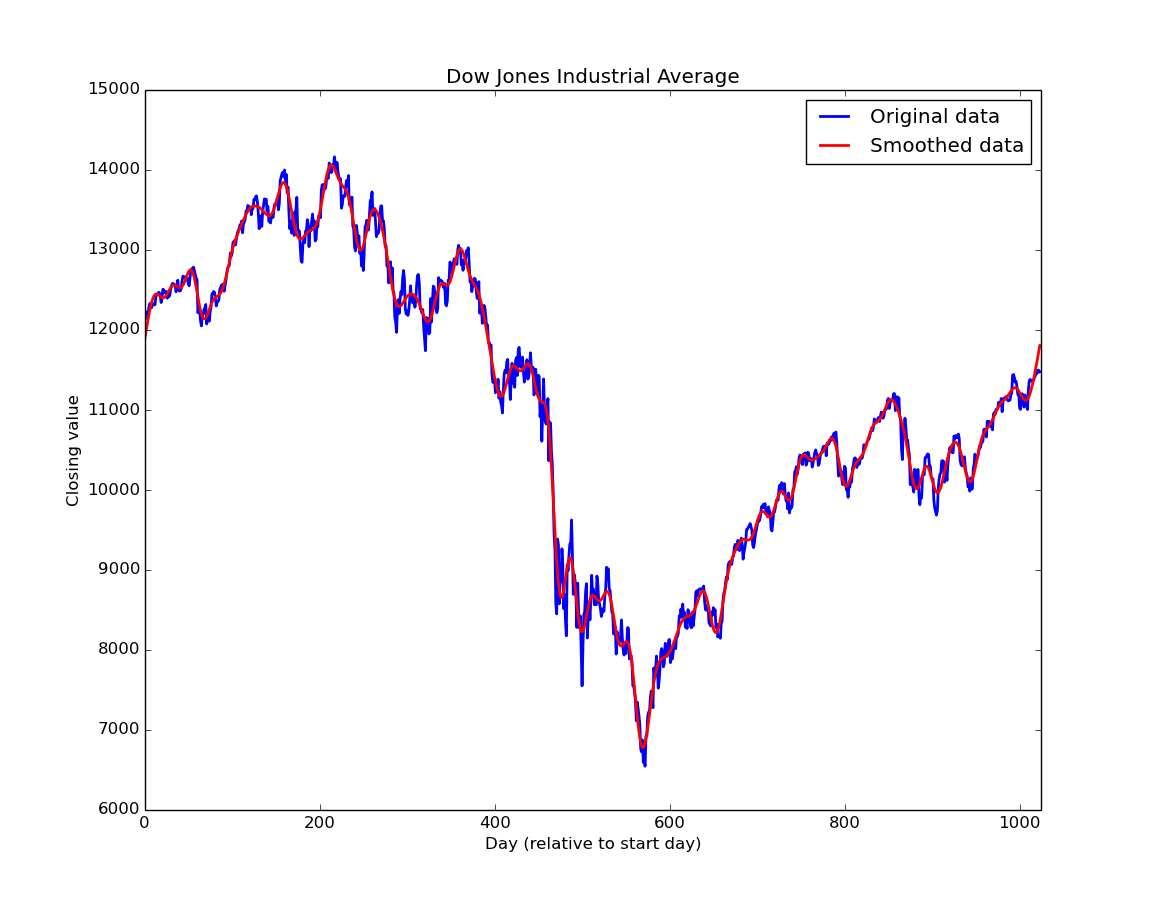
\includegraphics[width = \linewidth]{lab5q1.png}
\caption{}
\label{fig:q1}
\end{figure}

When all but the first few Fourier coefficients are set to zero, the data becomes smoothed. This makes sense, as higher Fourier coefficients correspond to higher frequency sinusoids. So by setting these coefficients to zero, we are removing the small scale variations and keeping only the overall shape determined by the low frequency sinusoids.

\section{Question 2}

\begin{figure}[H]
\centering
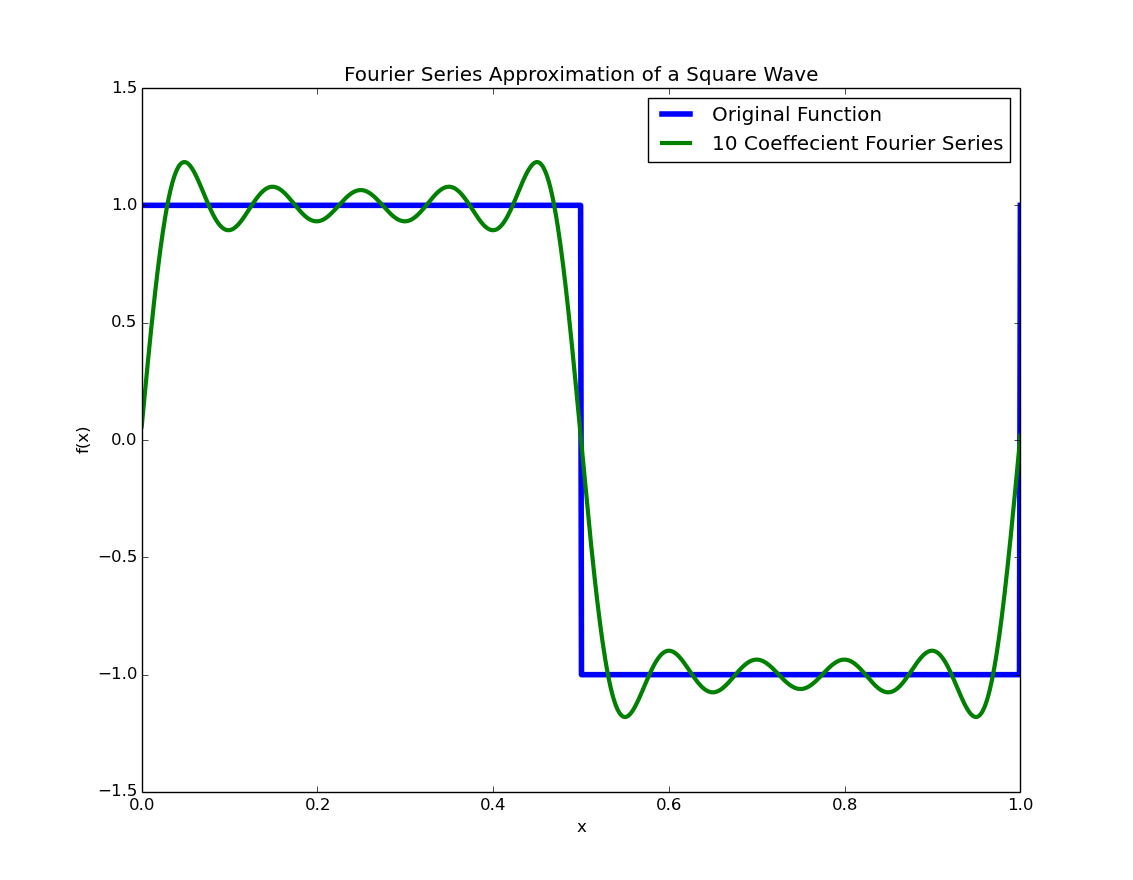
\includegraphics[width = \linewidth]{lab5q2.png}
\caption{}
\label{fig:q2}
\end{figure}

There are artifacts in our result that wiggle it away from the original signal because we discard some of the Fourier coefficients. This results in a less accurate approximation of the original function. Since a true Fourier has a infinite number of sine waves, approximating our function with just 10 sine waves results in a lot of artifacts. As the number of sine waves increases, the approximation is better, but there will still be artifacts at x=0.5, where the square wave is instananeously vertical. This feature is impossible to recreate with smooth sine waves, so there will always be some artifacts at the edges of the wave, unless infinite sinusoids are used.

\section{Question 3}

\subsection{Part a)}

\begin{figure}[H]
\centering
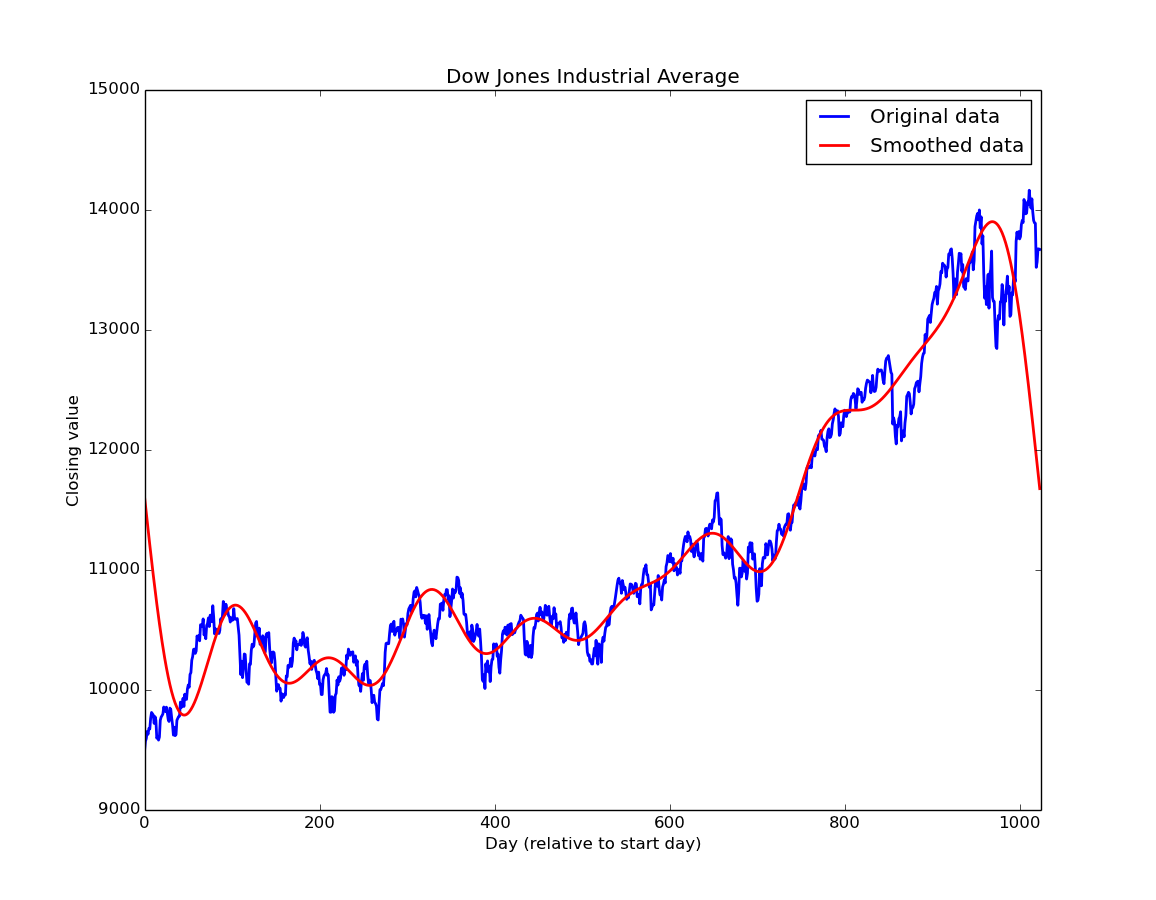
\includegraphics[width = \linewidth]{lab5q3a.png}
\caption{}
\label{fig:q3a}
\end{figure}

\subsection{Part b)}

\begin{figure}[H]
\centering
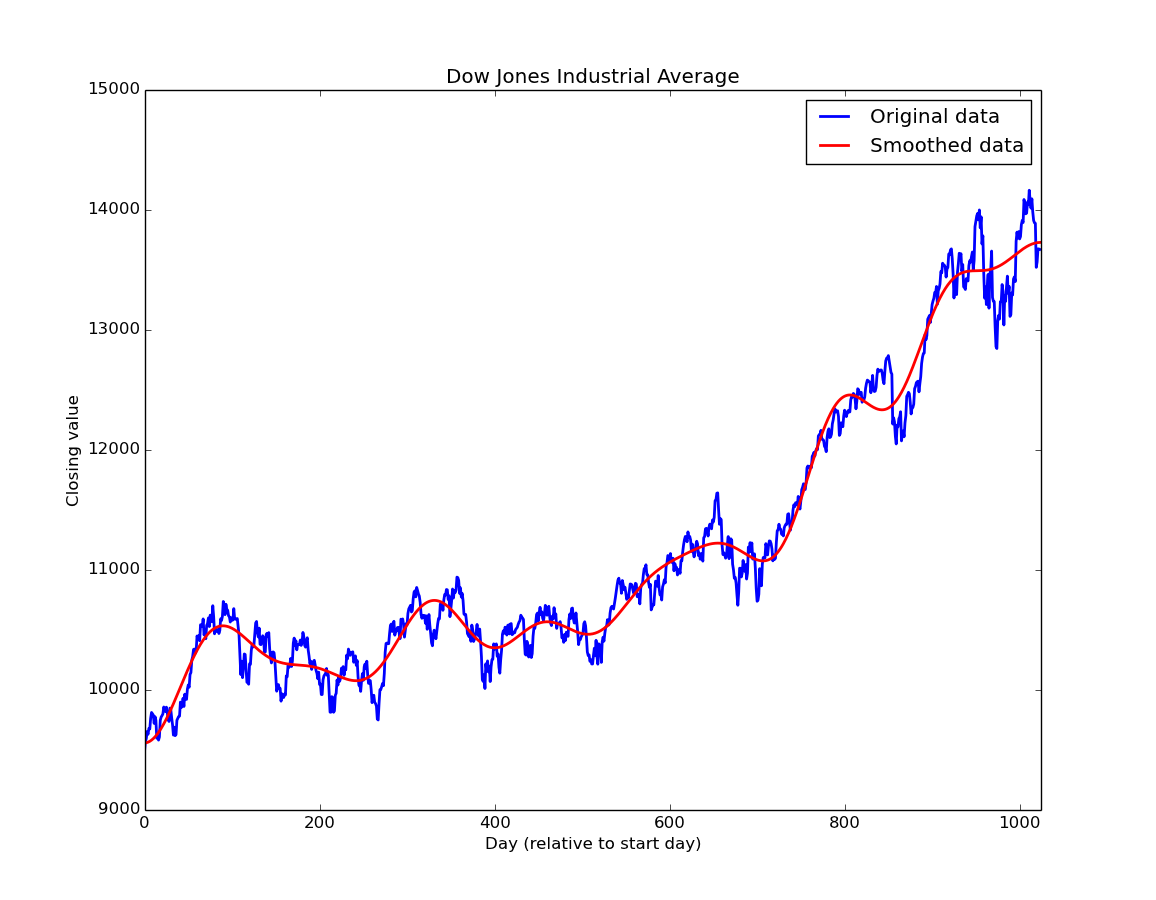
\includegraphics[width = \linewidth]{lab5q3b.png}
\caption{}
\label{fig:q3b}
\end{figure}

\section{Question 4}

\begin{figure}[H]
\centering
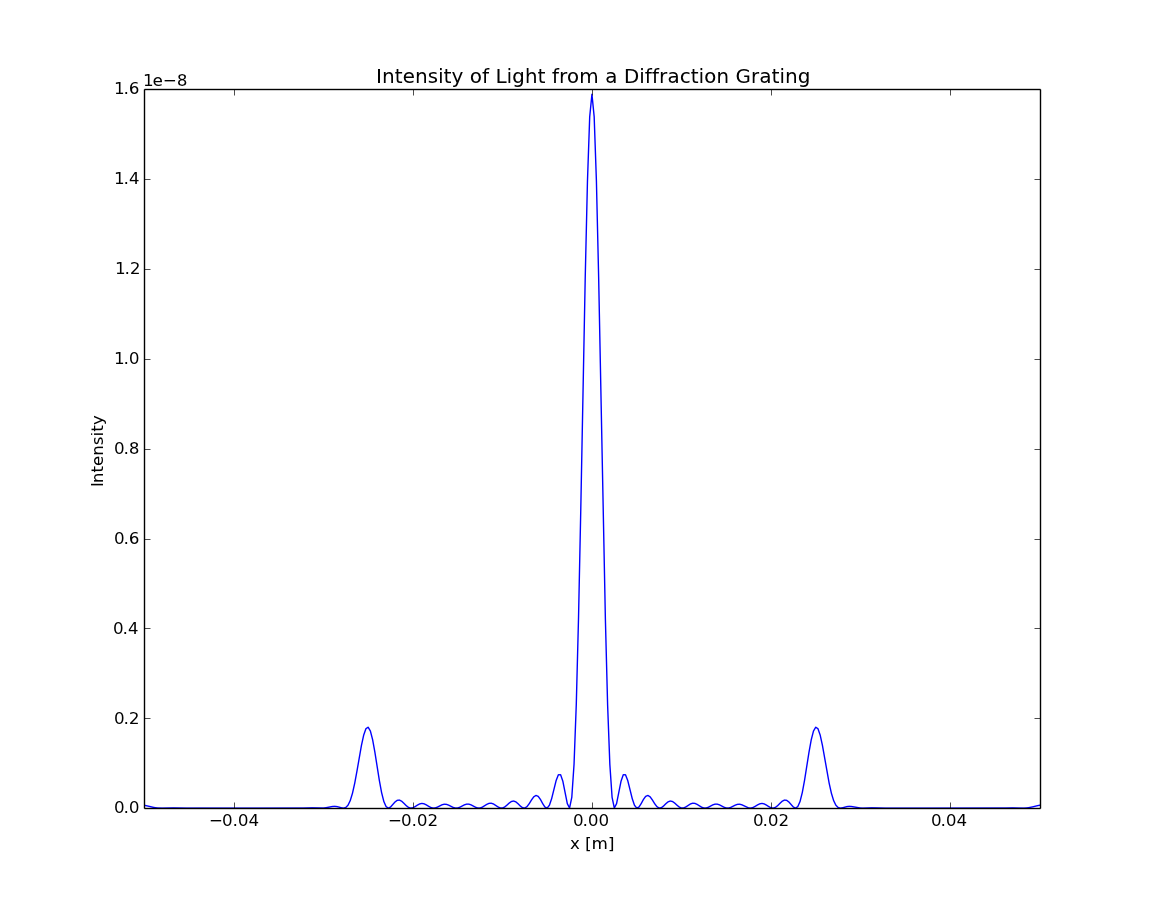
\includegraphics[width = \linewidth]{lab5q4.png}
\caption{}
\label{fig:q4}
\end{figure}

\section{Question 5}

\begin{figure}[H]
\centering
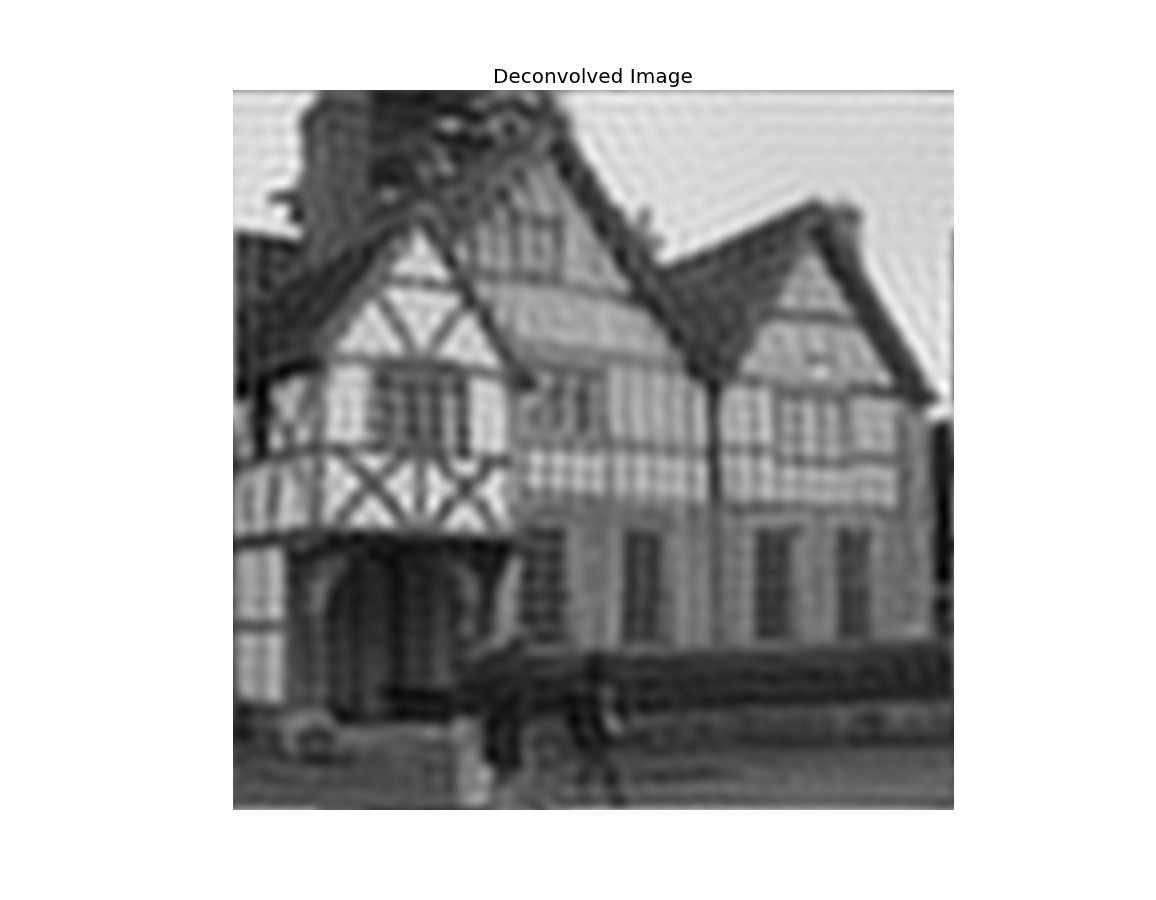
\includegraphics[width = \linewidth]{lab5q5.png}
\caption{}
\label{fig:q5}
\end{figure}

\end{document}





